\section{Plattform Hadoop"=Benchmark}
\label{sec:hadoopBenchmark}

\citeauthor{Zhang2016} haben im Rahmen ihrer gesamten Forschungsarbeit an der Selfbalancing"=Komponente darüber hinaus auch die Open"=Source"=Plattform \textbf{Hadoop"=Benchmark} entwickelt\footnote{\url{https://github.com/Spirals-Team/hadoop-benchmark}}.
Sie dient zur einfachen und schnellen Ausführung eines Hadoop"=Clusters und wurde speziell zum Einsatz in der Forschung erstellt.
Dadurch kann sie auch mit geringem Aufwand an eigene Bedürfnisse angepasst werden.

Zur Ausführung des Clusters wird die Virtualisierungs"=Software Docker\footnote{\url{https://www.docker.com/}} und das dazugehörige \emph{Docker Machine} genutzt.
Durch die Virtualisierung wird für jeden Hadoop"=Node eine Docker"=Machine gestartet, auf der der Hadoop"=Node wiederum in einem Docker"=Container ausgeführt wird.
Verbunden werden die Nodes dabei mithilfe eines \emph{Docker" Swarm}s\footnote{\url{https://docs.docker.com/engine/swarm/}}.

\begin{figure}[h]
    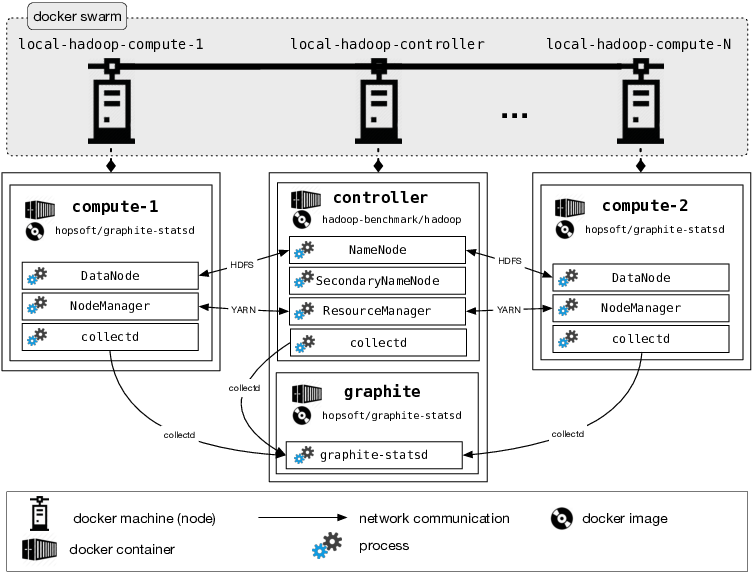
\includegraphics{./resources/hadoopBenchmarkArch.png}
    \caption[High"=Level"=Architektur von Hadoop"=Benchmark]
    {High"=Level"=Architektur von Hadoop"=Benchmark (entnommen aus \cite{abb:hadoopBenchmarkArch})}
    \label{fig:hadoopBenchmarkArchitecture}
\end{figure}

Docker"=Machine ist keine komplette Virtualisierungs"=Software, sondern nutzt hier VirtualBox\footnote{\url{https://www.virtualbox.org/}}, um virtuelle Maschinen zu starten, die mit dem Betriebssystem \emph{Boot2Docker} ausgestattet sind.
Boot2Docker ist eine leichtgewichtige Linux"=Distribution, auf der Docker bereits vorinstalliert ist \cite{DockerMachineGettingStartedVm}.

Mit \emph{Graphite}\footnote{\url{https://graphiteapp.org/}} ist zudem ein Monitoring"=Tool enthalten, mit dem die Systemwerte wie CPU- oder Speicher"=Auslastung des Clusters überwacht und analysiert werden kann.
Jeder Hadoop"=Container enthält dazu das Tool \emph{collectd}\footnote{\url{https://collectd.org/}}, was das Monitoring des Containers auf Systemebene übernimmt und die Daten an den Graphite"=Container übermittelt.

Da mithilfe der Plattform auch unterschiedliche Hadoop"=Konfigurationen ausgeführt werden können, ist die Plattform in mehrere Szenarien unterteilt.
Jedes Szenario stellt eine Hadoop"=Konfiguration dar, die vollständig angepasst werden kann.
Jedes Szenario enthält daher eine \emph{Dockerfile}, aus der die Docker"=Images und -Container erstellt werden, weitere für Hadoop benötigte Daten und Einstellungen, sowie dazugehörige generelle Einstellungen des Szenarios.
Die Plattform enthält bereits mehrere Szenarien, \uA Hadoop in der Version 2.7.1 ohne Anpassungen sowie ein darauf basierendes Szenario mit der Selfbalancing"=Komponente.
Aufgrund eines der Kernkonzepte von Docker, wonach Docker"=Images auf einem passenden, bereits vorhandenen Images aufbauen können bzw. sollten \cite{DockerdevBestPractice}, ist es möglich, neue Szenarien basierend auf bereits vorhandenen zu entwickeln.

Zum Starten des Clusters ist ein Script enthalten, welches basierend auf dem zu nutzenden Szenario das Cluster in der entsprechenden Konfiguration startet.

Die Plattform Hadoop"=Benchmark enthält auch einige Benchmark"=Anwendungen:

\begin{itemize}
    \item Hadoop Mapreduce Examples
    \item Intel HiBench\footnote{\url{https://github.com/intel-hadoop/HiBench}}
    \item \ac{SWIM} \footnote{\url{https://github.com/SWIMProjectUCB/SWIM}}
\end{itemize}

Die Benchmarks werden ebenfalls mithilfe der in der Plattform enthaltenen Scripte gestartet.
Hierbei besitzt jeder Benchmark ein eigenes Script, das den Benchmark in einem Docker"=Container startet und so dem Cluster zur Ausführung übersendet.

%Eine Besonderheit bildet der SWIM"=Benchmark, welcher sehr Ressourcenintensiv ist und daher auf einem \emph{Single Node Cluster}, also einem kompletten Hadoop"=Cluster auf nur einem physischem Host, sehr zeitintensiv sein kann.
%Beim Intel HiBench"=Benchmark sind die verfügbaren Anwendungen dagegen in verschiedene \emph{Worklaods} wie \emph{Machine Learning} unterteilt.
%Hierbei können die enthaltenen Anwendungen einzeln oder als ganze Workloads auf dem Cluster ausgeführt werden.
%Einige der Hibench"=Workloads bzw. Anwendungen basieren auf den Mapreduce Examples, welche wiederum voneinander unabhängige Beispielanwendungen für Hadoop darstellen.

Genauere Informationen zu den in der Plattform enthaltenen Benchmarks sind in \cref{sec:appOverview} erläutert.
